\documentclass{article}

\usepackage{graphicx}
\usepackage{amsfonts}
\usepackage{amssymb}
\usepackage{amsmath}

\graphicspath{ {fisica-generale/assets/} }

\begin{document}

\section{Statica}

La statica si occupa dello studio delle forze in situazioni di equilibrio.

\subsection{Forze}

Una forza è "l'entità" che causa una variazione del moto di un corpo.
Matematicamente, una forza è descritta da un vettore $\vec{F}$.

\begin{description}
    \item["Intensità"] corrisponde a $|\vec{F}|$
    \item[Direzione e verso] corrispondono alla direzione e verso di $\vec{F}$
\end{description}

\noindent
Quando si applicano due forze allo stesso oggetto, si può descrivere la forza risultante come la somma dei vettori delle due forze.

\begin{description}
    \item["Vettori liberi"] vettori definiti da modulo, direzione e verso
    \item["Vettori applicati"] vettori in cui, oltre a modulo, direzione e verso, si specifica anche il punto di applicazione
\end{description}

\noindent
È importante descrivere le forze come vettori applicati perchè il punto di applicazione è rilevante.

\subsection{Momento di una forza}

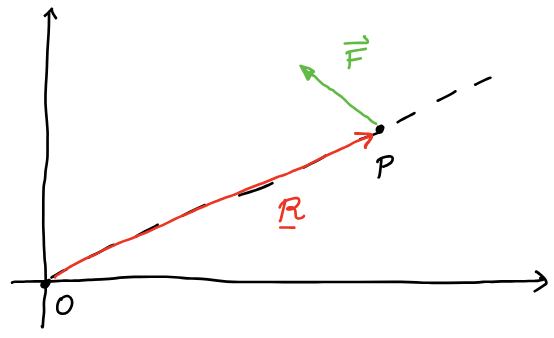
\includegraphics[width=\columnwidth]{esempio-momento-della-forza}

\noindent
Dati i punti $O$, $P$ e $\vec{R}$, si definisce il momento della forza $\vec{F}$ (che agisce su $P$) rispetto ad $O$ come:

$$
\vec{M} = \vec{r} \wedge \vec{F}
$$

\subsection{Quiete}

Un punto è in quiete in un sistema di riferimento, se ha una velocità nulla in ogni istante.

\subsection{Equilibrio}

Se un sistema di punti inizialmente in quiete rimane in quiete (anche se agiscono forze), si dice che si trova in uno stato di equilibrio.
Si parla di equilibrio stabile se "piccole variazioni" dal sistema portano a piccoli spostamenti, altrimenti l'equilibrio è instabile.

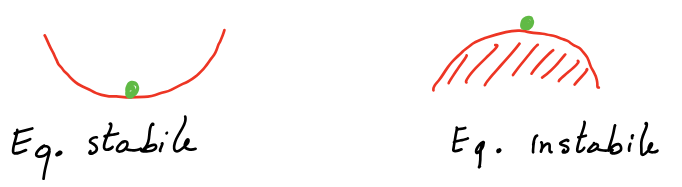
\includegraphics[width=\columnwidth]{equilibrio-stabile-e-instabile}

\subsection{Enunciato principale della statica}

Condizione necessaria e sufficiente affinchè un insieme di punti (o un "corpo esteso") sia all'equilibrio è che la risultante di tutte le forze sia nulla e che il momento totale delle forze sia nullo.

$$
\begin{matrix}
\sum_i \vec{F}_i = 0 \\
\sum_i \vec{r}_i \wedge \vec{F}_i = 0
\end{matrix}
$$

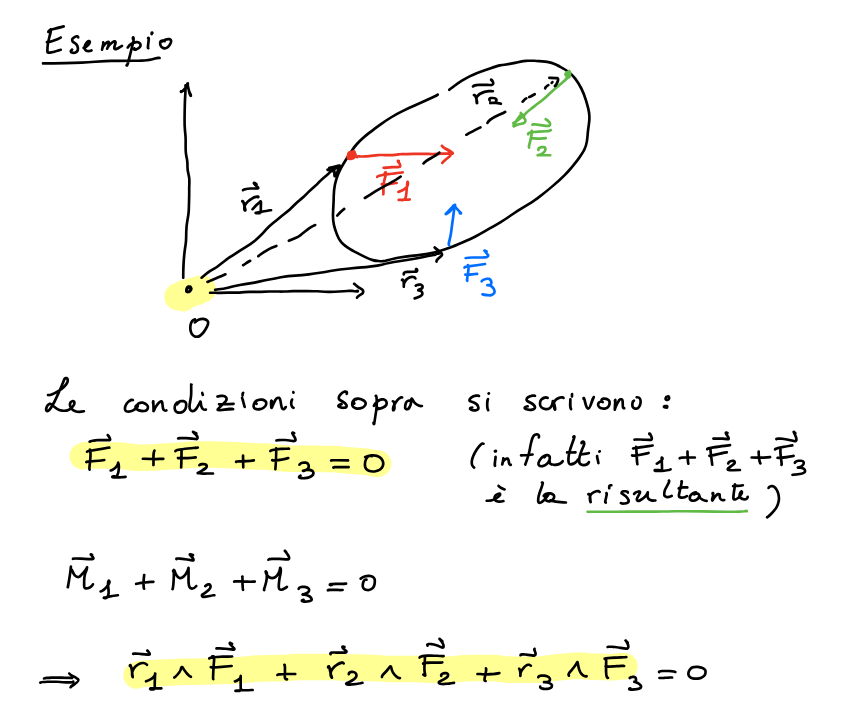
\includegraphics[width=\columnwidth]{esempio-enunciato-principale-della-statica}

\subsection{Reazioni vincolari}

Si parla di reazioni vincolari quando ci sono dei vincoli.
Un vincolo è una condizione che rende inaccessibili al punto alcune porzioni dello spazio.\\

\noindent
esempio, il tavolo impedisce alla palla di accedere ai punti con $y < 0$:

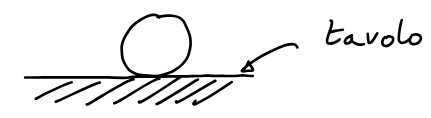
\includegraphics[width=\columnwidth]{esempio-reazione-vincolare}

\noindent
A livello microscopico, il tavolo si "deforma un po'", e possiamo pensarlo come un insieme di piccole molle.\\

\noindent
Un vincolo si dice liscio se non oppone resistenza rispetto ad un moto tangenziale alla superficie del vincolo ("no attrito").

\end{document}
